\documentclass[letterpaper,keeplastbox,twoside,10pt]{article}
\usepackage{usenix}
\usepackage{paralist}
\usepackage{wrapfig}
\usepackage{xspace}
\usepackage{comment}
\usepackage{epsfig}
\usepackage[hyphens]{url}
\usepackage{color}
\usepackage{times}
\usepackage{array}
\usepackage{ragged2e}
\usepackage{ifthen}
\usepackage{pifont}
\usepackage{amsmath}
\usepackage{tabularx}
\usepackage{makecell}
\usepackage{multirow}
\usepackage{changepage}
\usepackage{array,booktabs}
\usepackage{microtype}
\usepackage{subcaption}
\usepackage{caption}
\usepackage{booktabs}
\usepackage{placeins}
\usepackage{flushend}
\usepackage{multicol}
\usepackage{graphicx}
\usepackage{algorithm}
\usepackage{color,soul}
\usepackage[
bookmarks,bookmarksopen,
pdfstartview={FitH},
colorlinks,linkcolor={black},citecolor={black},
urlcolor={black}
]
{hyperref}

\addtolength{\belowcaptionskip}{-5pt}

\newcommand{\grumbler}[2]{\textcolor{red}{\bf #1: #2}}
% Add your own...
\newcommand\tab[1][1cm]{\hspace*{#1}}

\begin{document}

\title{\Large Hybrid Prefetcher using ISB and BO}
\author{\rm Yan Pei, Michael He\\The University of Texas at Austin}

\maketitle

% \pagenumbering{gobble}
\pagenumbering{arabic}

\tableofcontents

\newpage
\section{Introduction}
\label{sec:intro}

This is the final class project of cs395t-lin: \emph{Prediction Mechanism in Computer Architecture}. Our group, which consist of Yan Pei and Michael He, chose the project of hybrid prefetch design.

``Hybrid prefetcher'' means a prefetcher built on several other prefetchers. A hybrid prefetcher issues prefetch requests based on what its underlying prefetchers issue. In our project, we designed a hybrid prefetcher using irregualr steam buffer prefetcher(\emph{ISB})\cite{isbpaper} and best-offset prefetcher(\emph{BO})\cite{bopaper}.

In the execution of a program, access patterns, i.e. the stream of data address visited, can be divided into \emph{regular pattern} and \emph{irregular pattern}. For example, the access is regular when traversing a simple array, where addresses can be represented by a base PC and a fixed stride. The access is regarded as irregular when addresses can't be represented as above.  Traversing a link list is irregular, where address are ordered in pointer chasing manner. These two kinds of access pattens can occur alone or interleave with each other.

As for types of prefetchers, most of prefetchers can be divided into two groups: \emph{regular prefetcher}\cite{bopaper, sandboxpaper} and \emph{irregular prefetcher}\cite{isbpaper, ghbpaper, reinforcementlearning}.
They are good at prefetching their corresponding patterns but is either inaccurate or inefficient at the other pattern. Their advantages are complimentary.
%\emph{Regular prefetchers} prefetch regular patterns well while \emph{irregular prefetchers} are good at irregular pattern. These two kinds of prefetchers' advantage are complimentary.
Therefore, we construct our hybrid prefetcher by combining one \emph{regular prefetcher} and one \emph{irregular prefetcher}.
We pick \emph{ISB}\cite{isbpaper} as irregular prefetcher component and \emph{BO}\cite{bopaper} as regular prefetcher component.

  \subsection{Irregular Stream Buffer Prefetcher}
  \label{sec:isbintro}

  \emph{ISB}, which stands for Irregular Stream Buffer prefetcher, is a state of the art irregular prefetcher. It enjoys extremely good accuracy with fairly good coverage. It is an idea built on Global History Buffer(\emph{GHB})\cite{ghbpaper}.
In \emph{GHB}, access stream of one PC is stored in a link list, which is very inconvenient to traverse. Instead of using GHB, \emph{ISB} assigns access pattern buffer for every PC.
The key idea of \emph{ISB} is to use an extra level of indirection to translate arbitrary pairs of correlated physical address(PC local access stream) into consecutive address in a new structural address space(PC local access stream buffer), which is visible only to the \emph{ISB}.
This structural address space allows the \emph{ISB} to organize prefetching meta-data so that it is both temporally and spatially ordered, which produce technical benefits in terms of coverage, accuracy and memory traffic overhead.

  \subsection{Best Offset Prefetcher}
  \label{sec:bointro}

  \emph{BO}, which stands for Best Offset prefetcher, is one of the championships of regular prefetchers. \emph{BO} is actually built on \emph{Sandbox prefetcher}\cite{sandboxpaper}.
 The \emph{Sandbox prefetcher} uses simple hardware and was shown to be quite effective, while the timeliness is not considered.
 Thus many late prefetches are issued in the \emph{Sandbox prefetcher}.
 The \emph{BO} is an offset prefetcher with a new method that takes into account prefetch timeliness. Briefly, the \emph{BO} prefetch offset is updated at the end of every learning phase. Each learning phase consists of several rounds.
 During a round, each offset in the list is tested once, and each offset's score is incremented if a hit occur.
 After all the rounds are finished in one learning phase, the offset with the highest score will be selected as the offset of the next learning phase.

%here needs one general discrption

 \subsection*{}
 In this project we design a hybrid prefetching system that uses PC as a feature, to combine irregular and regular prefetchers.
We use two sets of experiments, \emph{Brute Force Seach} and \emph{Static Analysis}, to measure the headroom of hybrid prefetching system. The \emph{Brute Force Search} finds the optimal decision of each PC.  
The \emph{Static Analysis} builds a offline heuristic that makes PC decisions closest to \emph{Brute Force Search}. 
Then this offline heuristic is used as a guide for \emph{Dynamic Hybrid Prefetcher (DHP)}.
The experiment results show that the DRAM bandwidth is a strong factor to affect headroom. On 6.4GB/s bandwidth, the headroom has on average 12\% speedup over naive hybrid prefetcher and our DHP can achieve 6\% of it. \par

 The rest of the report are organized as follows. Section \ref{sec:motivation} demonstrates the motivation of the project. Section \ref{sec:designflow} shows the design flow of our research process, detailedly describes our two headroom designs: brute force search and static analysis. Section \ref{sec:headroom} analyzes the result of headroom experiments and how the result should guide our real design. Section \ref{sec:ourdesign} will give the solution of our design and the result are evaluated in section \ref{sec:result}.
 
 
 

\newpage
\section{Motivation}
\label{sec:motivation}
As mentioned in section \ref{sec:intro}, the pros and cons are list in the follwing table \ref{table:regVsirreg}. Regular prefetchers are good at prefetching regular patterns while prefetching irregular patterns inaccurately. on the other hand, irregular prefetchers are good at prefetching irregular patterns while prefetching regular patterns inefficiently. Obviously, the advantage and disadvantage of these two kinds of prefetchers are complimentary. One straightforward idea is to identify regular patterns and irregular patterns during execution and apply corresponding prefetcher to issue prefetches.

\begin{table}[ht!]
\centering
\begin{tabular}{cccll}
\cline{1-3}
\multicolumn{1}{|c|}{}                     & \multicolumn{1}{c|}{Regular Access Pattern}             & \multicolumn{1}{c|}{Irregular Access Pattern}          &  &  \\ \cline{1-3}
\multicolumn{1}{|c|}{Regular Prefetcher}   & \multicolumn{1}{c|}{Accurate}              & \multicolumn{1}{c|}{{\color[HTML]{FE0000} Inaccurate}} &  &  \\ \cline{1-3}
\multicolumn{1}{|c|}{Irregular Prefetcher} & \multicolumn{1}{c|}{{\color[HTML]{FE0000} Inefficient}} & \multicolumn{1}{c|}{Accurate} &  &  \\ \cline{1-3}
\end{tabular}
\caption{Regular Vs. Irregular}
\label{table:regVsirreg}
\end{table}

  \subsection{Irregular Vs. Regular}
  \label{sec:irrVsre}
  Here we will show the performance graph of one regular benchmark and one irregular benchmark. In Fig.\ref{fig:regVsirreg}, \emph{libquantum} is a regular benchmark while \emph{omnetpp} is sort an irregular benchmark. We can see that, though \emph{ISB} and \emph{BO} have similar accuracy but \emph{BO}'s coverage is better, result in much more speedup than \emph{ISB}'s. That's why we call irregualr prefetchers are inefficient in detecting regular patterns. On the other hand, \emph{ISB} is much better than BO for benchmark \emph{omnetpp}. \emph{BO} even causes negative coverage because of huge cache pollution. This example shows that choosing right prefetcher for one kind of access pattern is crucial to improve benchmark performance.
  \begin{figure}[ht!]
	  \centering
	  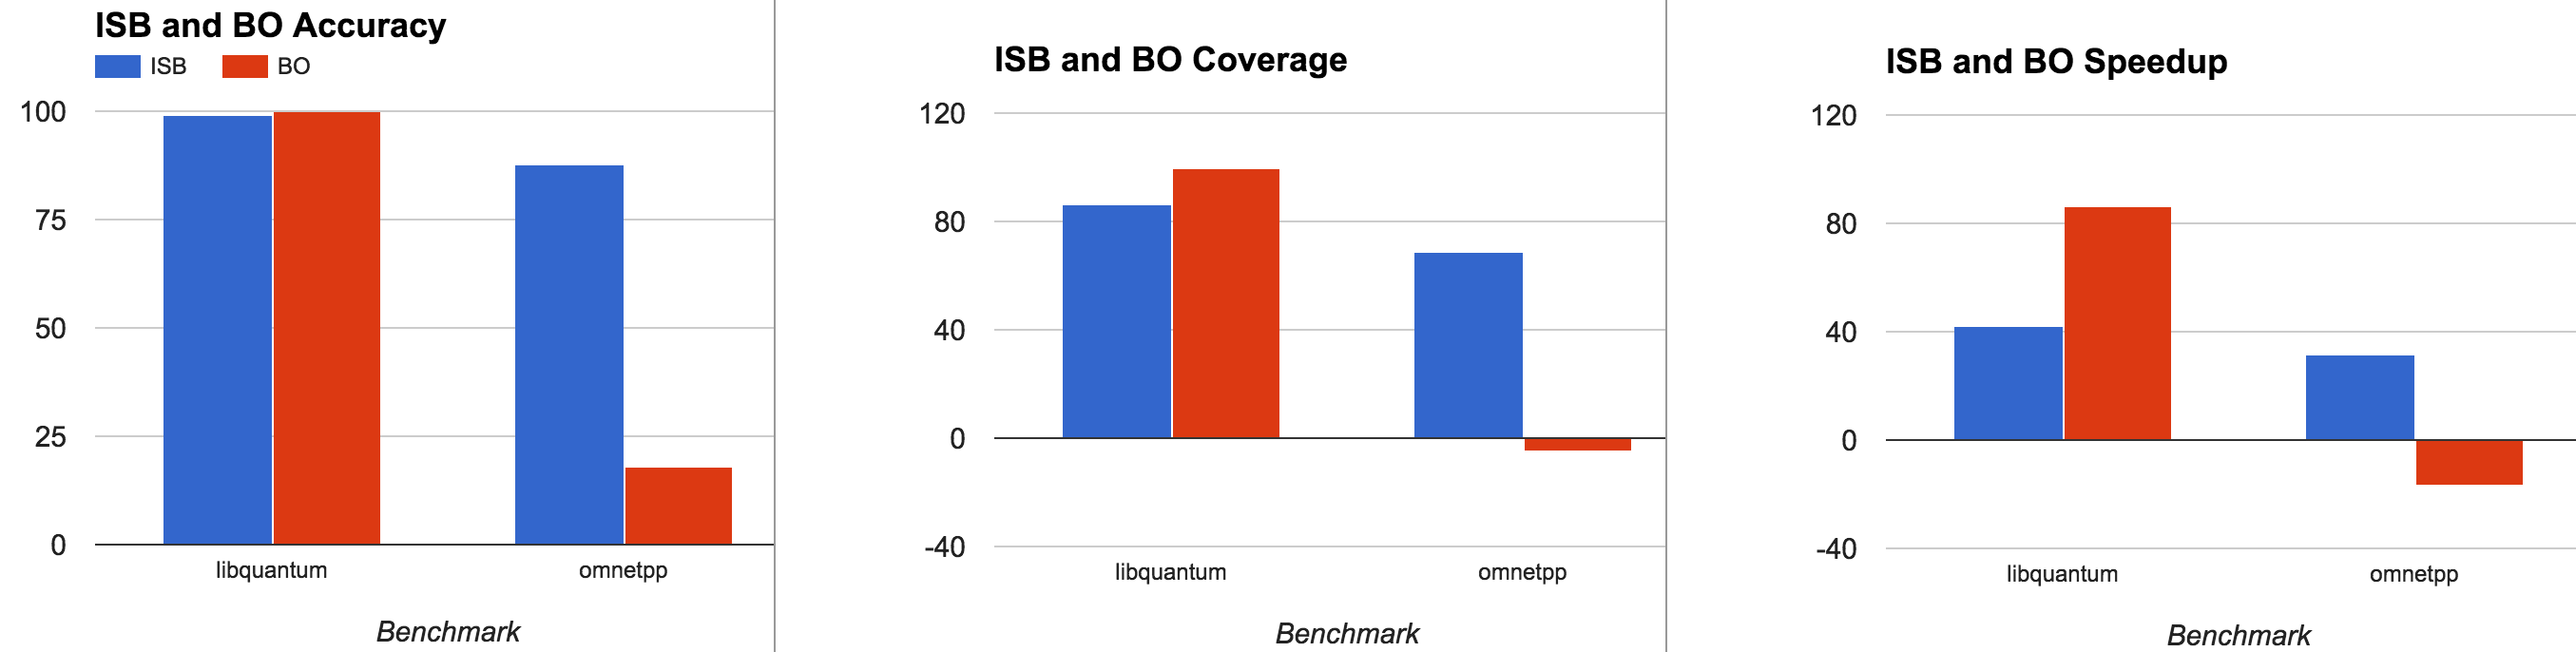
\includegraphics[width=1.0\textwidth]{images/isbvsbo.png}
	  \caption{\emph{ISB} and \emph{BO} performance comparision}
	  \label{fig:regVsirreg}
  \end{figure}


  \subsection{Naive Hybrid Prefetcher Vs. \emph{BO}\&\emph{ISB}}
  \label{sec:naivehy}
  One may ask a question after reading \ref{sec:irrVsre}: then why not issuing prefetches from both prefetchers? We call hybrid prefetcher with this behavior as \emph{naive hybrid prefetcher, or NHP}.
  \begin{figure}[ht!]
	  \centering
	  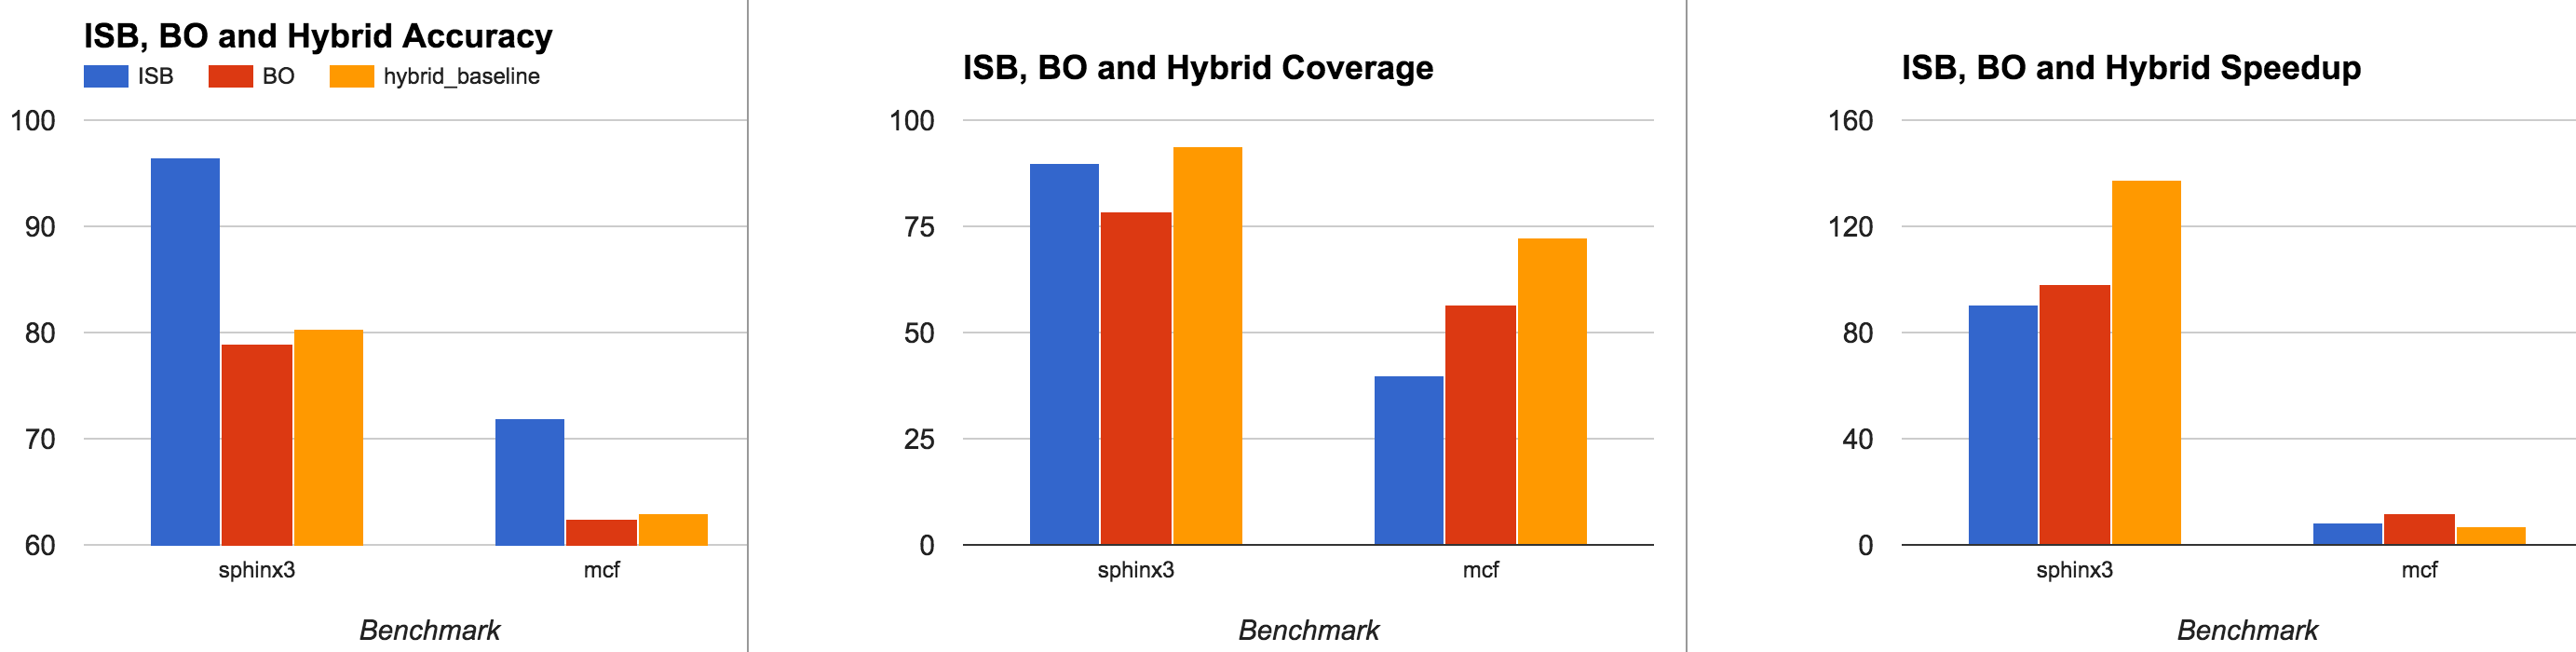
\includegraphics[width=1.0\textwidth]{images/hybridVssingle.png}
	  \caption{\emph{Naive Hybrid} and \emph{ISB, BO} performance comparision}
	  \label{fig:hybridVssingle}
  \end{figure}

  Well, it works when resource is enough rich, such as huge cache, huge memory bandwidth and so on. If these are limited, \emph{NHP} may cause huge memory pressure and cache pollution due to large number of inaccurate prefetches. In Fig.\ref{fig:hybridVssingle}, we give an example when \emph{NHP} works and when it doesn't. For benchmark \emph{sophinx3}, it is not memory intensive. The figure shows that the accuracy of \emph{ISB} is much higher than \emph{NHP}'s while \emph{NHP}'s coverage is much higher. It means that \emph{NHP} issued much more useless prefetchers to the cache. However, \emph{NHP}'s speed is still much better than \emph{ISB}'s. On the other hand, for benchmark \emph{mcf}, \emph{ISB} still has higher accuracy and lower coverage. However, this time, \emph{NHP}'s speed up is lower than \emph{ISB}'s. The possible reasons that a \emph{NHP} results in poor performance are listed below.

  \begin{itemize}
    \item Memory bandwidth is limited
    \item Memory request buffer size is limited
    \item Cache size is limited
    \item Cache pollution
  \end{itemize}

  \subsection{Previous Solution}
  \label{sec:PrevSol}
  previous solution

  \subsection{Our Goal}
  \label{sec:goal}
  Our design of hybrid prefetcher should do prefetches smartly. Idealy, if our hybrid prefetcher can utilize \emph{BO} and \emph{ISB}'s advantage well while avoiding the influence of their disadvantages, the hybrid prefetcher should enjoy better accuracy, coverage and speedup. The rest of the report are organized as follows. Section \ref{fig:design_flow} described the way we design our research process. Section \ref{sec:headroom} analyzes the result of headroom experiments and how the result should guide our real design. Section \ref{sec:ourdesign} will give the solution of our design and the result are evaluated in section \ref{sec:result}.

\newpage
\section{Headroom Experiment}
\label{sec:headroom}
In this section, headroom experiment results are analyzed to guide our dynamic hybrid prefetcher design. In section \ref{sec:headroomanalysis} we will talk about the potential of our design and the difference between two headroom test. In section \ref{sec:memorybandwidthissue}, one of the most influential factor, memory bandwidth, will be discussed in detail. Some other insights will be revealed in section \ref{sec:otherinsights}.

  \subsection{Headroom Result Analysis}
  \label{sec:headroomanalysis}

  \begin{figure}[ht!]
	   \centering
	   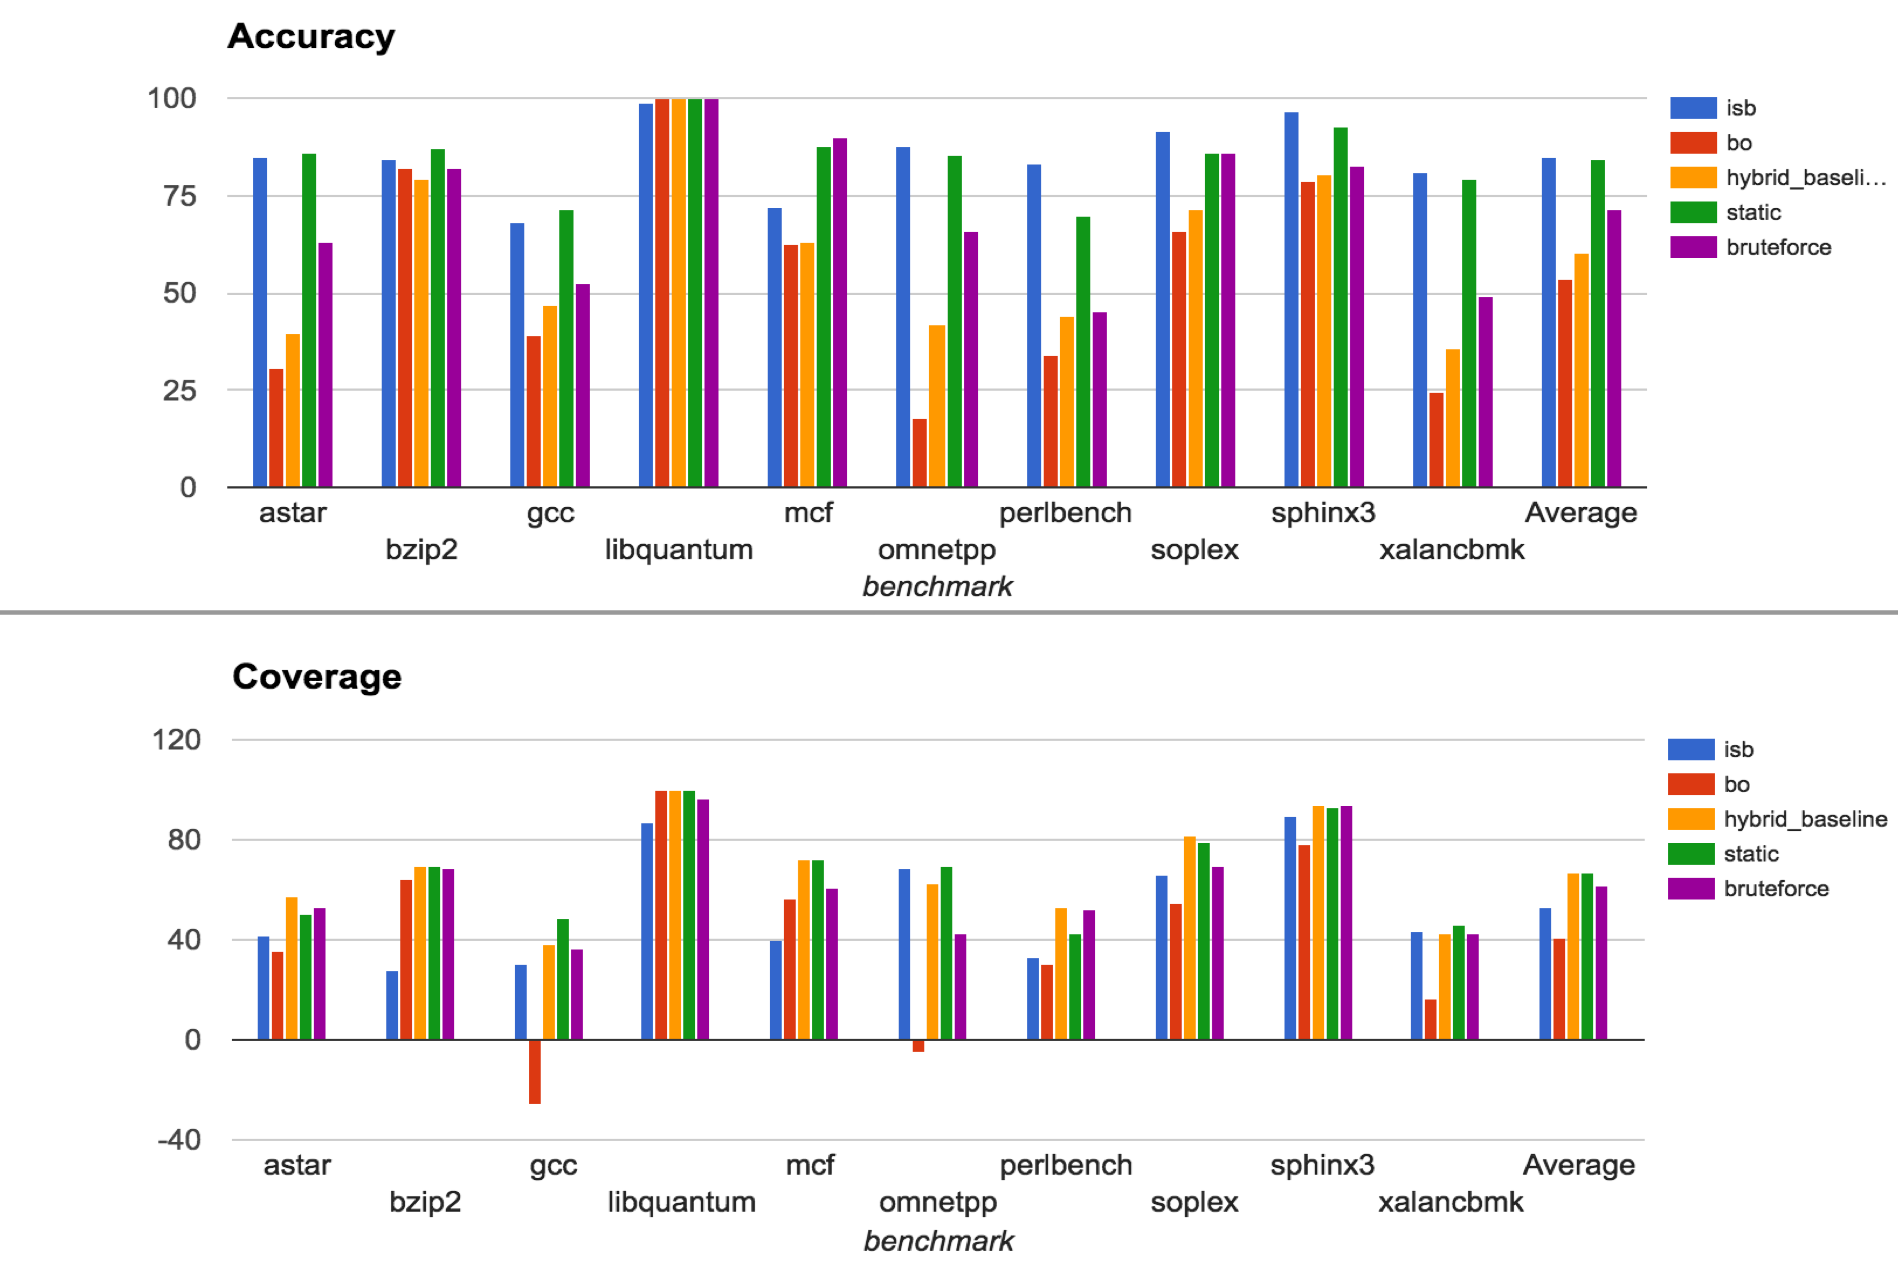
\includegraphics[width=1.0\textwidth]{images/headroom_acc_cov.png}
	   \caption{Headroom accuracy and coverage performance}
	  \label{fig:headroom_acc_cov}
  \end{figure}

  In Fig.\ref{fig:headroom_acc_cov}, the accuracy and coverage performance of \emph{ISB, BO, NHP, Static Analysis} and \emph{Brute Force Search}. Comparing \emph{NHP} with \emph{ISB, BO}, we found that the accuracy of \emph{NHP} is significantly lower than \emph{ISB}'s, while its coverage is higher than \emph{ISB}. It indicate that \emph{NHP} issued much more prefetches than \emph{ISB} or \emph{BO}. For \emph{static analysis} part, it achieves similar accuracy with \emph{ISB}'s, and similar coverage with \emph{NHP}'s. This is understandable since static analysis focus on static data files, making wise decisions is the only thing it can do. The \emph{Brute Force Search} method focuses on speedup most. Therefore, its accuracy and coverage performance are not as good as the static ones'. Because we use \emph{SNIPER} as our simulator, the accuracy and coverage keep the same even we change the bandwidth since no prefetch is abandoned.

  Though accuracy and coverage are good metrics for evaluating prefetchers. The most import performance metric is speedup. The speedup numbers of different bandwidth are shown in Fig.\ref{fig:headroom_speedup}. Note that here and in all the later figures, the speedup is comparing to system with no prefetcher. Interestingly, we got results of different shapes when the bandwidth is different. \emph{ISB} has higher speedup during low bandwidth while \emph{BO} has higher during high bandwidth. The reason is that high bandwidth wouldn't give much punishment to useless prefetch while low bandwidth does. For \emph{NHP}, in both configuration it enjoys higher speedup. However, the headroom of 6.4GB/s bandwidth is more than 11\%, while only 4\% in 12.8GB/s bandwidth case. Another point worth attention is that though static method enjoys higher accuracy and coverage than the brute force one, \emph{Brute Force Search} still has better speed up. Intuitively, it is because some prefetches shouldn't have been issued by \emph{Static Analysis} due to high memory pressure at that point. The detail reason will be explained in section \ref{sec:memorybandwidthissue}.

  In our later evaluation, we will choose 6.4GB/s as our bandwidth since the headroom is quite encouraging in that case.

  %higher accuracy and coverage doesn't imply better speedup.

  \begin{figure}[ht!]
	   \centering
	   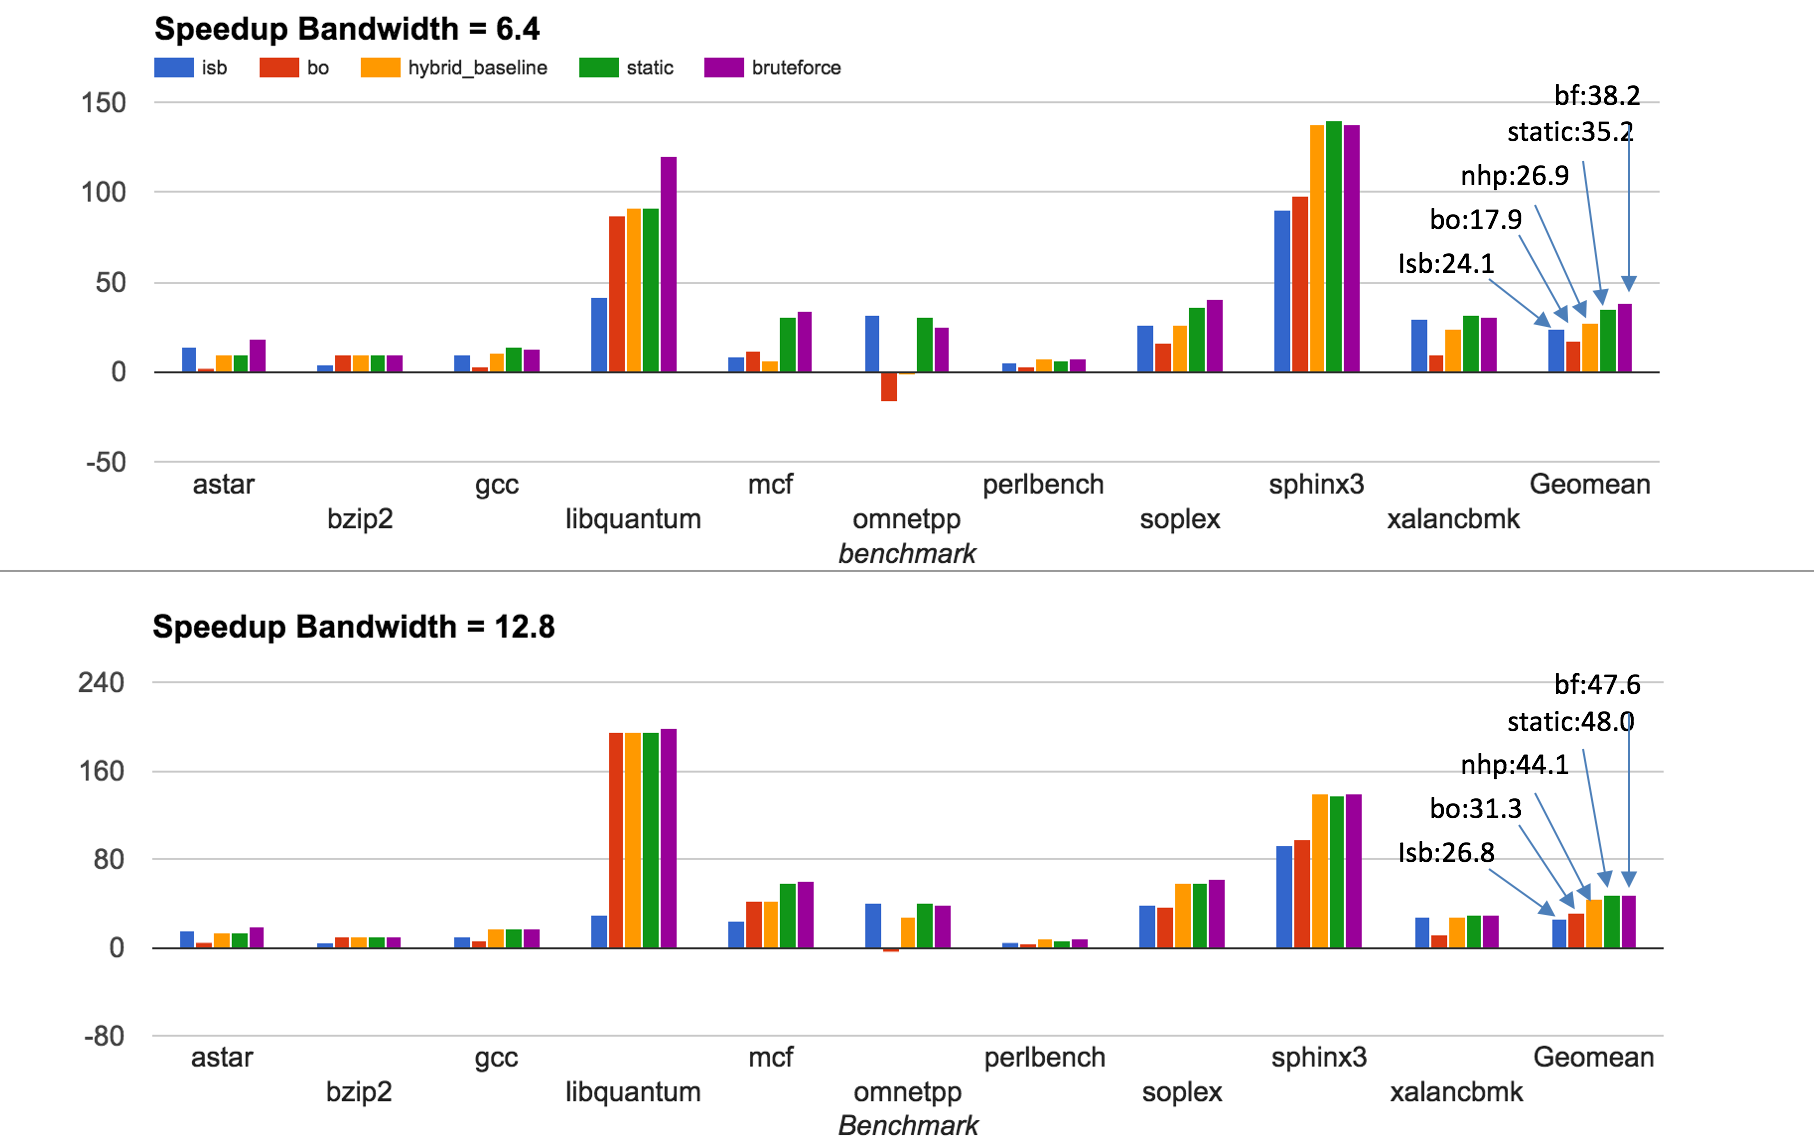
\includegraphics[width=1.0\textwidth]{images/headroom_speedup.png}
	   \caption{Headroom speedup under different memory bandwidth}
	  \label{fig:headroom_speedup}
  \end{figure}

  \subsection{Memory Bandwidth Issue}

  \label{sec:memorybandwidhissue}
  In Fig.\ref{fig:headroom_speedup}, the headroom of high bandwidth 12.8 GB/s is from NHP 44.1\% to static 48\%, it has about 3.9\% headroom. On low bandwidth 6.4 GB/s, the headroom is from NHP 26.9\% to BF 38.2\%, headroom is 11.3\%. 
  The figure shows that the headroom of hybrid prefetching system is highly related to memory bandwidth, and it is consistent with our previous discussion: hybrid prefetching system is limited by the amount of shared resources. 
  The less resources it has, the more headroom it can achieve.\par
  

    \begin{figure}[h]
	   \centering
	   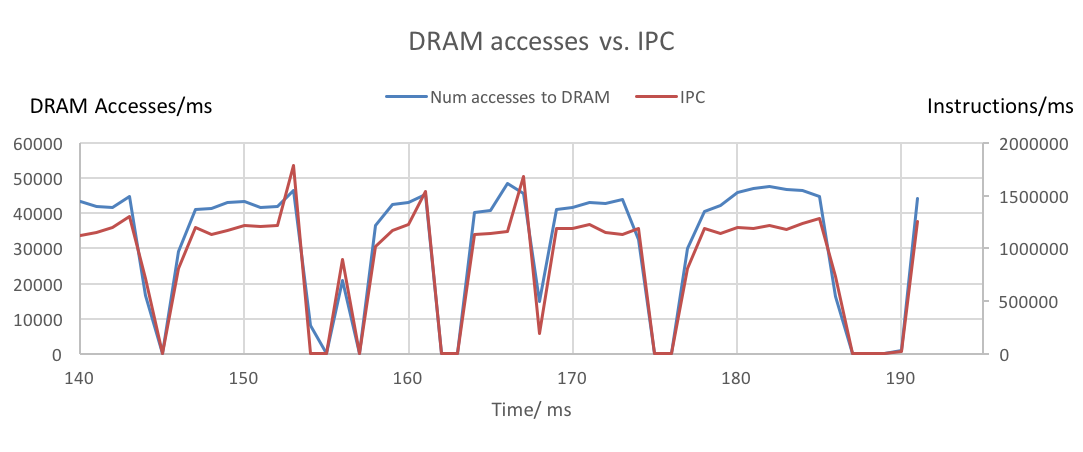
\includegraphics[width=0.8\textwidth]{images/bandwidth_IPC.png}
	   \caption{DRAM accesses vs IPC}
	  \label{fig:bandwidth_IPC}
  \end{figure}
  \begin{figure}[h]
	   \centering
	   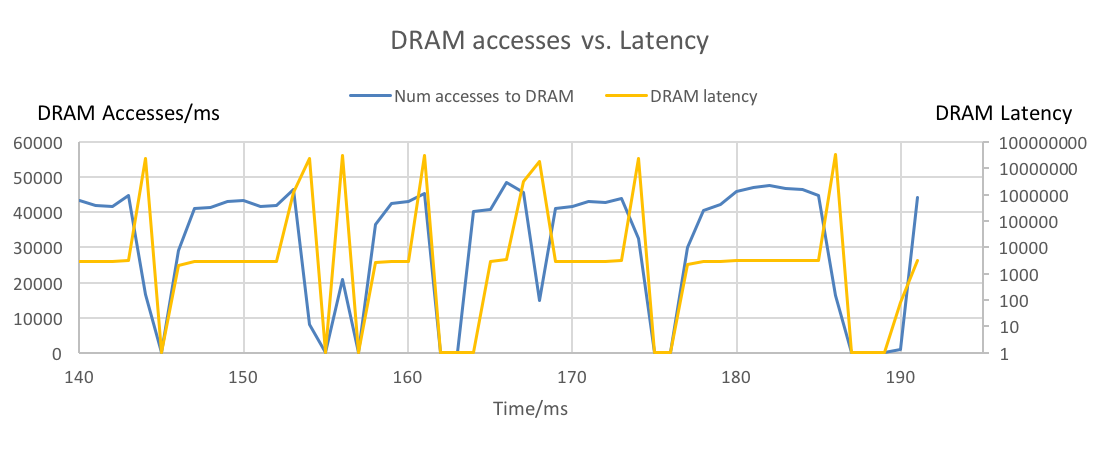
\includegraphics[width=0.8\textwidth]{images/bandwidth_latency.png}
	   \caption{DRAM accesses vs DRAM latency}
	  \label{fig:bandwidth_latency}
  \end{figure}
In this part we will discuss in detail how the memory bandwidth influences our performance, and how we can deal with it.\par
Fig.\ref{fig:bandwidth_IPC} and Fig.\ref{fig:bandwidth_latency} shows bandwidth, IPC and memory latency from benchmark \emph{astar} sim point 1 from 140ms to 192ms. The blue lines in both graphs are numbers of DRAM accesses per ms, which denotes the bandwidth usage. Red line is the number of executed instructions per ms, which denotes IPC. Yellow line is the sum of latency of all DRAM accesses per ms. X axis is the time line.\par
In Fig.\ref{fig:bandwidth_IPC}, DRAM accesses and IPC almost overlap. This indicates that at the low points, the benchmark program is stalled and DRAM doesn't receive any more request. For those low points in Fig.\ref{fig:bandwidth_latency}, latency increases a lot at the low points. Note that the latency Y axis is in log scale, the latency actually increases four to five magnitudes at those moments. The reason why the peak points of yellow is a little before the low points of blue is that, the sniper simulator calculates the latency of an access at the moment it is issued, not at the moment it returns.\par
 We can draw conclusions from these two figures that: 1) On some benchmarks, programs are occasionally stalled due to limited memory bandwidth and this is a significant issue to the performance. 2) Memory bandwidth should be considered in the hybrid prefetching system.  In our current headroom experiments, PCs make static decisions offline and never change decisions during execution. When we implement dynamic hybrid system, bandwidth usage is a factor to control the prefetching degree of prefetchers. \par


  \subsection{Some other insights}
  \label{sec:otherinsights}
  Besides memory bandwidth factor, we have some other insights about these headroom experiments.
  \begin{itemize}
    \item Performance is input dependent. A well built benchmark set is important
    \item The brute force experiments are not optimal, but they can still show the preference of each PC.
    \item In the headroom experiment, PCs’ decisions are made offline and not changed during execution. And we have up to 12\% speedup headroom. If PC can make dynamic decisions, we may have more speedup.
    \item Memory bandwidth pressure affects the prefetch performance a lot. It needs to be considered and measured in dynamic hybrid prefetching system.
  \end{itemize}

\newpage
\section{Design Flow}
\label{sec:designflow}

\begin{figure}[ht!]
	\centering
	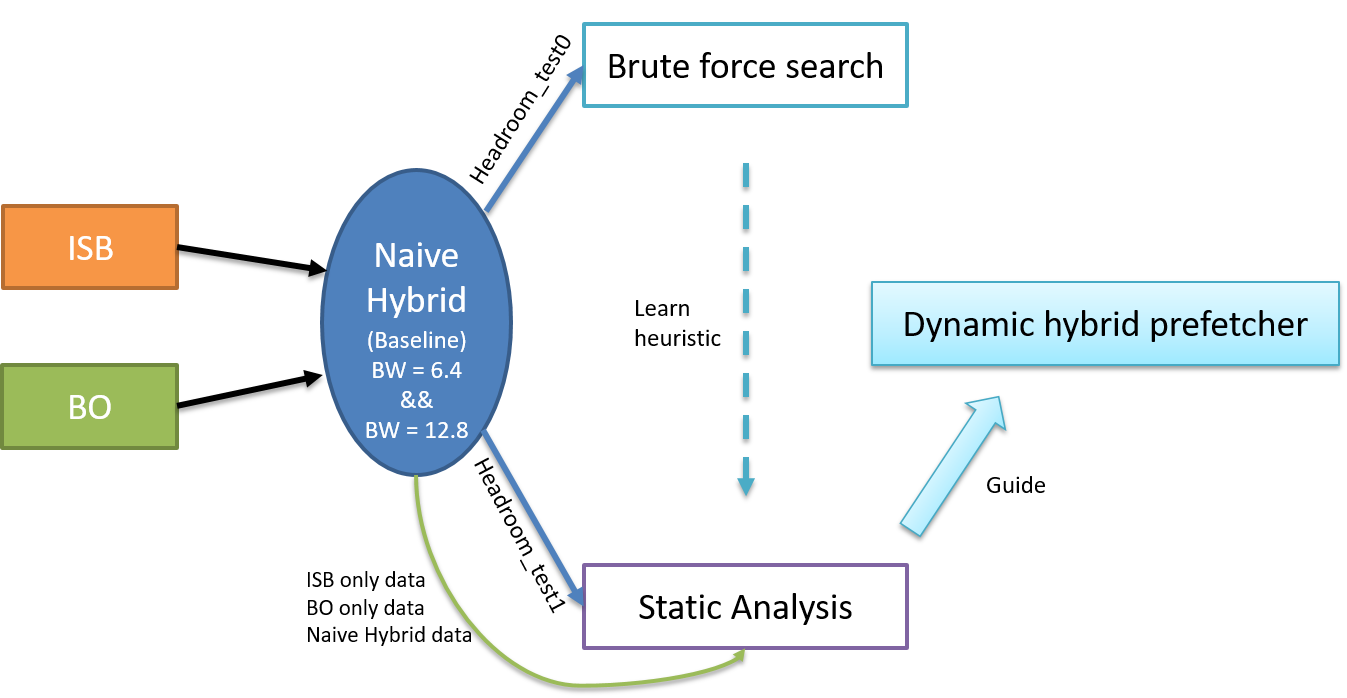
\includegraphics[width=1.0\textwidth]{images/design_flow.png}
	\caption{Design flow}
	\label{fig:design_flow}
\end{figure}

Based on the introduction and motivation we demonstrated above, we design our headroom experiments and ``smart'' hybrid prefetcher system in Fig.\ref{fig:design_flow}.

First, we will evaluate the individual performance of \emph{BO}, \emph{ISB} and \emph{NHP}. Note that here we measure performance using two different memory bandwidth configuration. 12.8 represents high memory bandwidth 12.8 GB/s and 6.4 represents low memory bandwidth 6.4 GB/s. The \emph{Brute Force Search} and \emph{Static Analysis} are both offline headroom designs which will be described in the following two sections. Briefly, \emph{Brute Force Search} tries each choice on each PC, and finds out the best decisions and optimal headroom. Static Analysis comes up with a heuristic. It uses the statistics of each PC from ISB, BO and naive hybrid experiments as input, and builds a strategy that makes decisions closest to \emph{Brute Force Search} thus achieves best speedup. Finally the Static Analysis guides the design of our final hybrid prefetch system, which will be explained in section \ref{sec:ourdesign}.

  \subsection{Brute Force Search}
  \label{sec:bruteforcesearch}

  In this part, we will first illustrate why we need a \emph{Brute Force Search} to find the headroom of PC localization. Then we show how Brute Force Search headroom experiment is designed. \par

  \subsubsection{Metric to measure a PC}
  \label{sec:metricPC}

  It is known that accuracy and coverage are two good metrics \cite{yalepaper} to measure the performance of a prefetcher. They are calculated as follows:
  \begin{equation}
  Accuracy = \frac{prefetch\ hits}{total\  prefetched}
  \end{equation}
  \begin{equation}
  Coverage = \frac{prefetch\ hits}{total\ prefetch\ hits + total\ misses}
  \end{equation}

  Similarly we can define accuracy and coverage of a trigger PC:
  \begin{equation}
  PC\ Accuracy = \frac{prefetch\ hits\ by\ this\ PC}{prefetches\ by\ this\ PC}
  \end{equation}
  \begin{equation}
  PC\ Coverage = \frac{prefetch\ hits\ by\ this\ PC}{total\ prefetch\ hits + total\ misses}
 \end{equation}

 \begin{figure}[ht!]
	\centering
	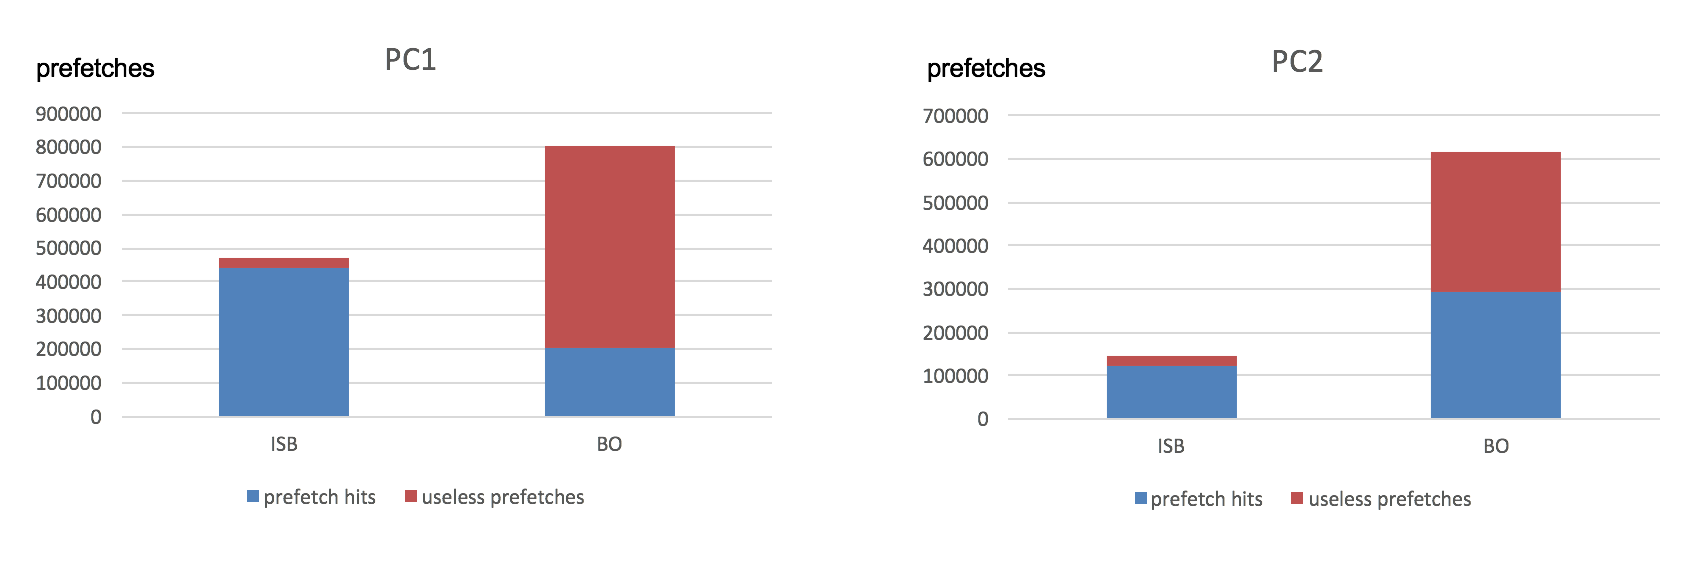
\includegraphics[width=1.0\textwidth]{images/metric.png}
	\caption{Hits and useless prefetches example}
	\label{fig:pcmetric}
\end{figure}

However, these two metrics from \emph{ISB} and \emph{BO} sometimes cannot determine the preference of a PC.
For example in Fig.\ref{fig:pcmetric}, on PC1, it is clear that ISB on this PC has higher accuracy and coverage, so the hybrid system should choose ISB. But on PC2, ISB has higher accuracy but BO has higher coverage, then it's hard to choose.
In terms of speedup, prefetch hits has positive contribution and useless prefetches has negative contribution.
On PC2, BO has more prefetch hits and more useless prefetches, so it's hard to infer its contribution is positive or negative only on this numbers.

    \subsubsection{Design of Brute Force Search}
    \label{sec:designBFS}
    Since the effect of accuracy and coverage of a PC to the overall performance is not clear, we design the Brute Force Search experiment to explore the space of PC's choices and find out the headroom. The steps are listed as follows. \par
    1) Choose several PCs with the main influence. For each pinpoint, we find out the PC with the most prefetches, denoted this number as MAX. Any PCs that has prefetches more than 5\% of MAX are chosen.\par
    2) Find the best decision for each PC. For each PC, run four experiments, respectively set its decision to ISB, BO, neither or both. \textbf{All other PCs are set to choose both}.\par
    3) Combine the best decisions of all PCs.\par
    Note that for the several PCs we consider, they can cover more than 95\% of total prefetches, so they can represent the prefetch charactaristic of a benchmark. \par
    Here the Brute Force Search design is not optimal. An optimal exploration should run all the possible choices over all PCs, i.e. $4^{n}$ experiments, n is the number of PC considered, which it is around 10 to 30.
    This exploration space is too large and needs too many experiments, so we take one step back and design this suboptimal search, which need 4*n experiments. Because it sets all non-considered PC to both, it's basically compare the four choices to all PCs choosing both, which might over estimate the bandwidth consumption. \par

  \subsection{Static Analysis}
  \label{sec:staticanalysis}
  Another path to know about headroom is to use static analysis method. The high level design flow is shown in Fig.\ref{fig:staticanalysis_flow}. The input for a benchmark are three files from \emph{ISB} only execution, \emph{BO} only execution and \emph{NHP} execution. In each performance file, it records the hits and prefetches issued by each PC. As described in Fig.\ref{fig:pcmetric}, some PC are easy to make decision but some are not. Here we come up with some heuristic from \emph{Brute Forse Search} to guide our decision making process. After going through the heuristic, each PC has a fixed decision over the whole benchmark execution: \emph{BOTH, NEITHER, ISB} and \emph{BO}.

  \begin{figure}[ht!]
	  \centering
	  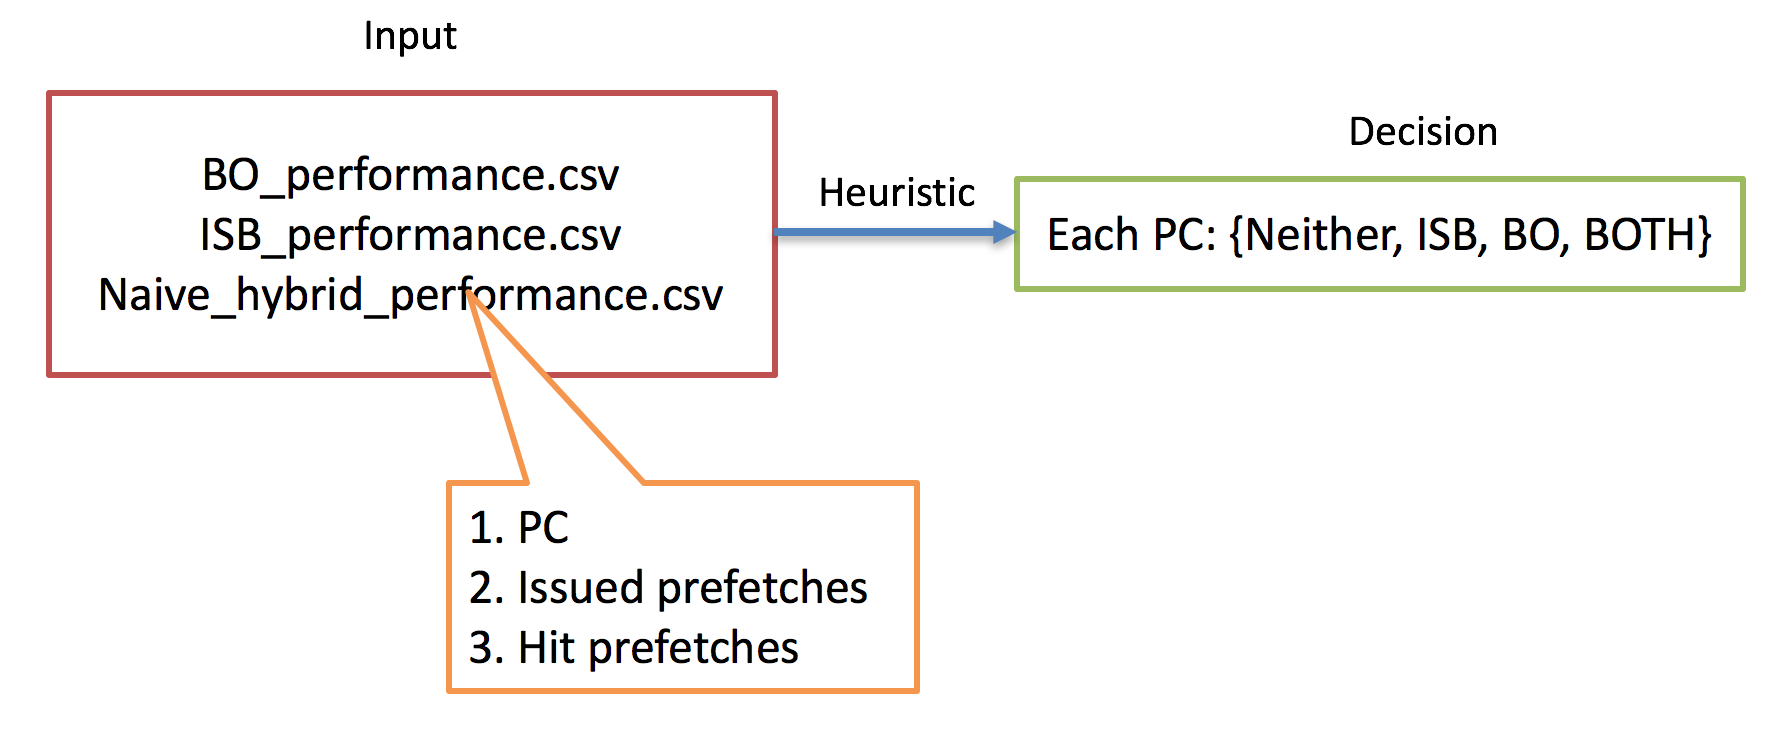
\includegraphics[width=0.8\textwidth]{images/staticanalysis_flow.png}
	  \caption{Static Analysis Design Flow}
	  \label{fig:staticanalysis_flow}
  \end{figure}


  \begin{figure}[ht!]
	  \centering
	  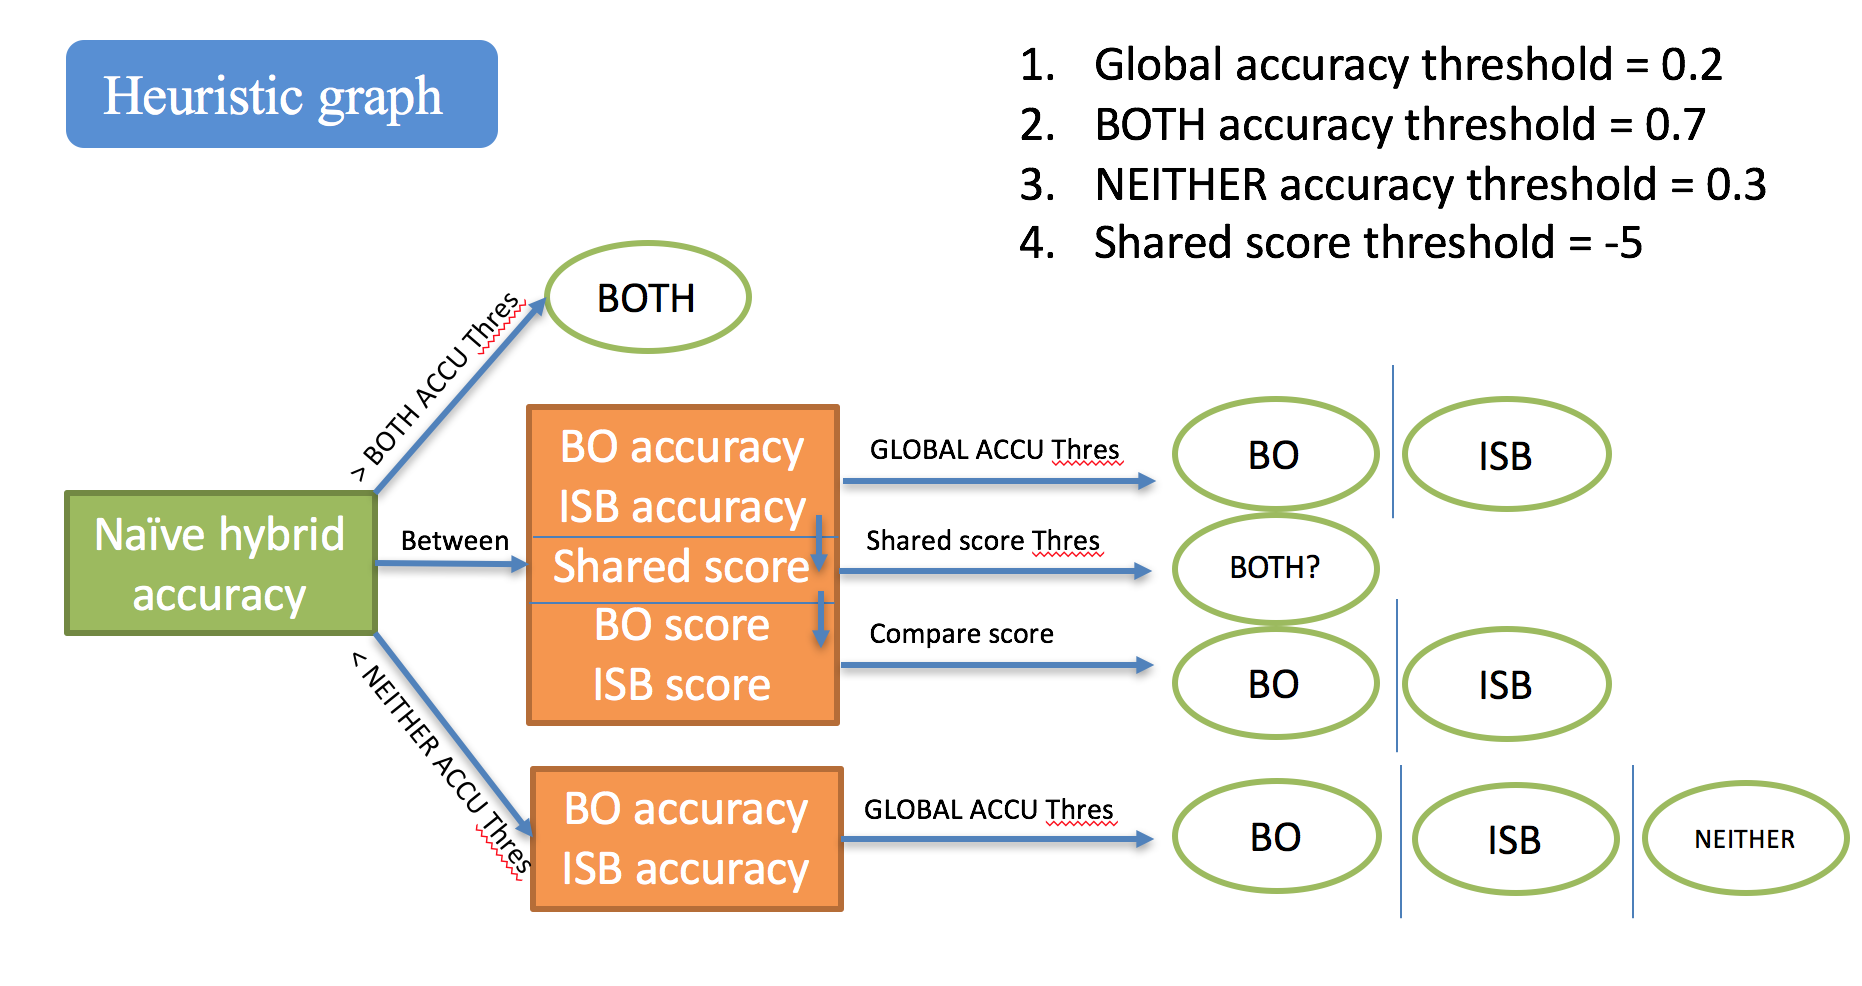
\includegraphics[width=0.8\textwidth]{images/heuristic_design.png}
	  \caption{Heuristic Design}
	  \label{fig:heuritic design}
  \end{figure}

  Here we will describle how our heuristic are designed in Fig.\ref{fig:heuritic design}. Four threshold are defined by user. \emph{Global Accuracy Threshold} set the lowest acceptable accuracy of one PC of any kind of prefetcher. \emph{BOTH Accuracy Threshold} determines when we should prefetch both. \emph{NEITHER Accuracy Threshold} determines when we should prefetch at most one of them. Last but not least, \emph{Shared Score Threshold} determines how should shared hits and shared prefetch affect the final decision. The decision process is list as follows.

  1) Compare \emph{NHP}'s accuracy with \emph{BOTH Accuracy Threshold}. If \emph{NHP}'s accuracy is higher than threshold, the hybrid prefetcher would choose both prefetches from \emph{ISB} and \emph{BO}.

  2) Compare \emph{NHP}'s accuracy with \emph{NEITHER Accuracy Threshold}. If \emph{NHP}'s accuracy is lower than threshold, the hybrid prefetcher would choose prefetches from either \emph{ISB}, or \emph{BO} or neither of them.

  3) Compare \emph{ISB}'s and \emph{BO}'s with \emph{Global Accuracy Threshold}, make decision when one meet the threshold and the the other does not. If both meet, go to step 4.

  4) Calculte the shared score. The shared score calculate how many shared hits and shared miss prefetch are made. Usually less share hits and more shared prefetches indicate better cache performance. The score is compared to \emph{Shared Score Threshold} in order to decide whether prefetch both or go to step 5. The score is calculated in equation.\ref{equ:shared_score}.

  \begin{equation}
  \label{equ:shared_score}
  shared\_score = shared\_hits - accuracy\_NHP * shared\_prefetch
  \end{equation}

  5) \emph{BO} score and \emph{ISB} score are defined in equation.\ref{equ:prefetcher_score}. The heuristic of this equation is to calulate the importance of hit and useless prefetches. Hits are more evaluated so we apply a coefficient to reduce the impact of useless prefetches. Finally, the hybrid prefetcher will pick the one with higher score.
  \begin{equation}
  \label{equ:prefetcher_score}
  score = hits - useless\_prefetch * (1 - accuracy\_NHP)
  \end{equation}

\newpage
\section{Experimental Methodology}
\label{sec:methodology}

We evaluate all our experiments using Sniper \cite{sniperpaper}, a next generation parallel, high-speed and accurate x86 simulator. Our simulation runs ten benchmarks from SPEC06 benchmark suite on a single core model. We disable the prefetching of L1 cache to make the access stream to L2 consistent. We use SimPoint sampling methodology. We simulate 250 million instruction on each SimPoint and simulate around 20 SimPoints on each benchmark. We now only simulate degree equals 1 for both ISB and BO. See Table \ref{table:config} for details. 
\begin{table}[ht!]
\centering
        \renewcommand{\multirowsetup}{\centering}  
        \begin{tabular}{|l|l|} 
        \hline  
        \multirow{2}{3cm}{benchmarks}   & {astar, bzip2, gcc, libquantum, mcf,omnetpp} \\
         \multirow{2}{3cm}{}  & {perlbench, soplex, sphinx3, xalancbmk} \\ \cline{1-2}
         \multirow{2}{3cm}{L1 cache}  & {size: 64kB, associativity: 8, block size = 64Bytes} \\
         \multirow{2}{3cm}{}  & {cache replacement policy: LRU, no prefetching} \\ \cline{1-2}
         \multirow{2}{3cm}{L2 cache}  & {size: 2048kB, associativity: 16, block size = 64Bytes} \\
         \multirow{2}{3cm}{}  & {cache replacement policy: LRU} \\ \cline{1-2}
         \multirow{2}{3cm}{DRAM }  
         	& {Latency: 54.4ns } \\ 
	 \multirow{1}{3cm}{}  & {per\ controller\ bandwidth = 6.4GB/s or 12.8GB/s} \\ \cline{1-2}
         \multirow{1}{3cm}{prefetchers}  & {ISB (degree = 1), BO (degree = 1)} \\ \cline{1-2}
        \hline 
        \end{tabular} 
\caption{Configuration}
\label{table:config}
\end{table}




\newpage
\section{Experimental Evaluation}
\label{sec:result}

The project

\newpage
\section{Conclusion and Future Work}
\label{sec:conclusion}

In this project we built a hybrid prefetching system that combines irregular and regular prefetchers, using PC localization. 
We ran two groups of headroom experiments, \emph{Brute Force Seach} and \emph{Static Analysis}. The \emph{Brute Force Search} finds the optimal decision of each PC.  
The \emph{Static Analysis} built a heuristic that uses PC statistics from ISB, BO and NHP as input, to make PC decisions closest to \emph{Brute Force Search}. 
Then this offline heuristic is used as a guide for dynamic hybrid prefetcher. 
The experiment results show that the headroom is highly related to DRAM bandwidth. On 6.4GB/s bandwidth, the headroom has on average 12\% speedup over NHP and our DHP can achieve 6\% of it. \par

We are now trying to add the bandwidth estimation to control the dynamic decisions of the hybrid system. 
As we have seen in the experiment result, currently the bandwidth-aware DHP even performs slower than DHP without it, and there is still a large gap between DH and the headroom. 
We think there are still some issues in our design of bandwidth-aware DHP. One issue might be the bandwidth estimation is incorrect. Using the number of DRAM accesses to measure bandwidth like in Section \ref{sec:memorybandwidhissue} is misleading. Because when the program is stalled by bandwidth, the simulator doesn't see any DRAM accesses issued and the bandwidth would be considered as free. However in fact, the bandwidth is fully occupied. The bandwidth would be our first step in future work. \par

The second will be adding the degree control to hybrid system. Now we only consider both ISB and BO with degree one. In the future it is necessary to increase the degree of ISB (BO's degree is at most 1).\par

\paragraph{Another Possible Direction}
During our headroom experiment design, we have been thinking about how to measure the preference of each PC. Finally our conclusion is that, because there is tradeoff between accuracy and coverage, it's difficult to decide the preference of a PC only by these two metrics. \par
Let's step back to the prefetching. There will be two possible results when a prefetch is issued: it finally hits and has positive contribution to performance, or it is finally useless and has negative contribution. Positive contribution is avoiding the latency to DRAM. Negative contribution is the occupation on bandwidth and pollution on cache. We take the positive contribution as benefit and negative contribution as cost. We can simply model the problem as\par

\begin{equation}
possible\ benefit = Benefit * Accuracy + Cost * (1-Accuracy)
\end{equation}

It would be convenient to determine which prefetcher is better if we have the benefit and cost. However, this is the most important part. The benefit and cost are dynamic and highly dependent on the system configuration, system status, benchmarks, simpoints etc. If we can estimate it using some machine learning techniques, it would be very useful. And the estimation here looks like related to the cost-aware OPT project.


\newpage
\section{Future work}
\label{sec:future}

No more future work please if no publication potential.


\newpage
\bibliographystyle{plain}
\bibliography{bibliography}

\end{document}
